\label{cap:metodologia}

\section{Descripción general del sistema}

El objetivo principal de este trabajo consiste en desarrollar un sistema de aprendizaje profundo capaz de detectar automáticamente lesiones del ligamento cruzado anterior (LCA) a partir de estudios de resonancia magnética (RM) de rodilla.

La metodología propuesta sigue un enfoque de clasificación directa de extremo a extremo (\textit{end-to-end}), evitando etapas explícitas de segmentación anatómica. Esta decisión se fundamenta tanto en criterios prácticos como clínicos. Por una parte, los modelos de segmentación requieren máscaras anotadas manualmente por especialistas, lo que supone un elevado coste temporal y computacional. Por otra, la clasificación directa permite preservar información contextual relevante de toda la articulación, incluyendo signos indirectos de lesión.

El pipeline general desarrollado puede dividirse en las siguientes etapas:

\begin{enumerate}
    \item Carga y normalización de estudios de resonancia magnética.
    \item Selección automática de cortes anatómicamente relevantes.
    \item Extracción de características mediante arquitecturas CNN y Transformer.
    \item Agregación de información entre cortes utilizando mecanismos de atención.
    \item Fusión multi-vista entre planos anatómicos.
    \item Clasificación binaria de lesión del LCA.
\end{enumerate}

La Figura~\ref{fig:pipeline_general} resume gráficamente este flujo de procesamiento, desde el volumen de RM de entrada hasta la predicción final de lesión del LCA.

\begin{figure}[H]
\centering
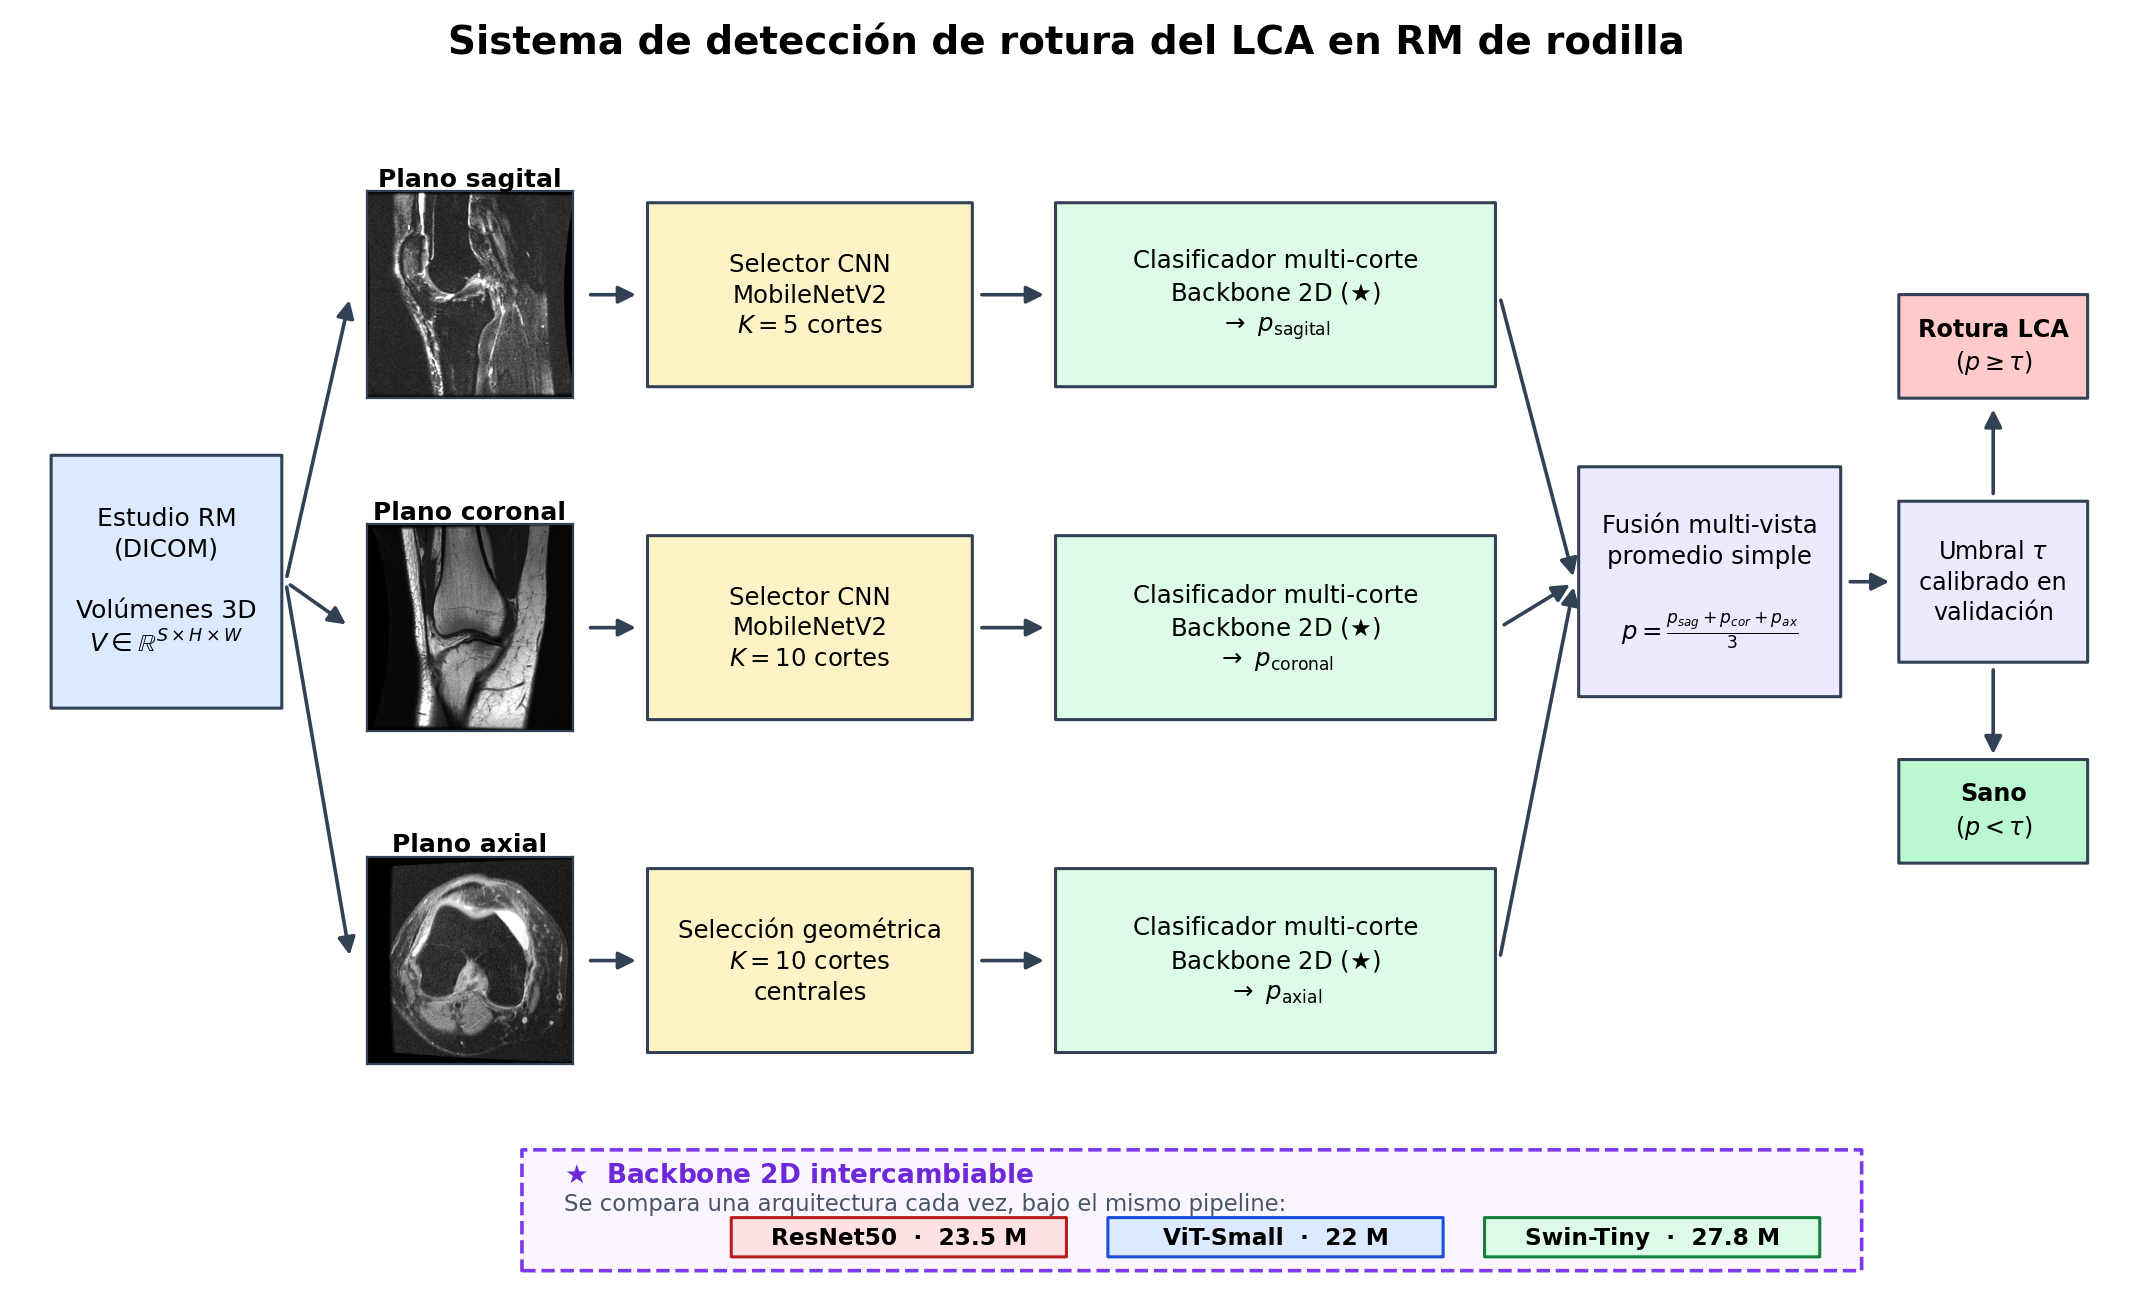
\includegraphics[width=0.92\textwidth]{figs/pipeline_general.png}
\caption{Esquema general del sistema propuesto: selección automática de cortes por plano, extracción de características mediante el \textit{backbone}, agregación de cortes mediante \textit{Attention Pooling} y fusión multi-vista de los tres planos anatómicos.}
\label{fig:pipeline_general}
\end{figure}

\section{Selección automática de cortes anatómicos}

Uno de los principales problemas asociados al procesamiento completo de volúmenes de RM es que únicamente una fracción reducida de los cortes contiene información anatómica relevante sobre el ligamento cruzado anterior.

Procesar todos los cortes incrementa:
\begin{itemize}
    \item el ruido visual,
    \item el coste computacional,
    \item y la redundancia espacial.
\end{itemize}

Por este motivo, en este trabajo se desarrolló un módulo propio de selección automática de cortes basado en una arquitectura \textbf{MobileNetV2}. En concreto, se entrenaron dos modelos independientes: uno específico para el plano sagital y otro específico para el plano coronal. Cada uno de ellos fue entrenado con sus propias etiquetas de relevancia anatómica, generadas de forma independiente para el plano correspondiente, de modo que el selector aprendiera qué cortes eran más informativos dentro de cada orientación.

La idea principal consiste en procesar los $N$ cortes que componen una serie de resonancia magnética y asignar a cada uno de ellos una puntuación de probabilidad asociada a la presencia o visibilidad del LCA en la imagen. A partir de estas puntuaciones, el sistema ordena los cortes de mayor a menor relevancia anatómica y selecciona automáticamente los $K$ cortes más informativos para el clasificador final.

De este modo, para cada estudio de RM el módulo actúa como una etapa previa de filtrado: recibe una secuencia completa de cortes sagitales o coronales y devuelve únicamente los 5 o 10 cortes con mayor probabilidad de contener información útil sobre el LCA, según el plano anatómico considerado. Esta selección no pretende diagnosticar la lesión, sino localizar las imágenes donde el ligamento es más visible o donde es más probable que aparezca información anatómica relevante para la clasificación posterior.

Esta estrategia se plantea como una contribución metodológica específica del trabajo. En lugar de utilizar únicamente cortes centrales o procesar todo el volumen completo, se introduce un selector aprendido que reduce la redundancia, limita el ruido visual y concentra el entrenamiento de los modelos diagnósticos en las regiones más relevantes. Hasta donde se ha revisado en el desarrollo de este trabajo, no se ha identificado una estrategia equivalente aplicada de esta forma en los trabajos comparados.

La Figura~\ref{fig:mri_slices_sagital} muestra un ejemplo real de los cortes sagitales seleccionados por el módulo para un estudio de RM, ordenados según la puntuación de relevancia anatómica asignada por el selector.

\begin{figure}[H]
\centering
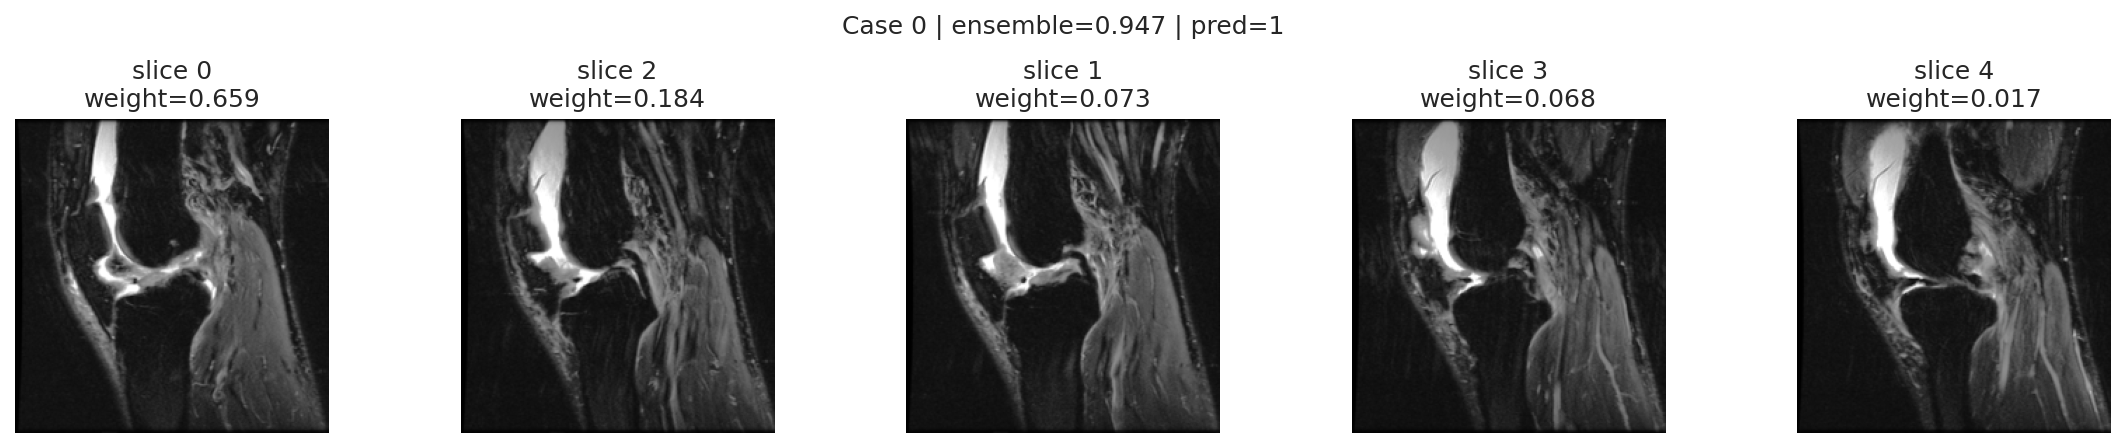
\includegraphics[width=\textwidth]{figs/mri_slices_sagital.png}
\caption{Ejemplo de cortes sagitales de un estudio de RM de rodilla seleccionados automáticamente por el módulo MobileNetV2, ordenados de mayor a menor probabilidad de contener información relevante del LCA.}
\label{fig:mri_slices_sagital}
\end{figure}

\subsection{Estrategias evaluadas}

Se analizaron distintas estrategias de selección:

\begin{itemize}
    \item \textbf{Center}: selección geométrica de los cortes centrales del volumen.
    \item \textbf{Random}: selección aleatoria utilizada durante entrenamiento como mecanismo de regularización.
    \item \textbf{CNN-Based}: selección automática basada en las puntuaciones generadas por MobileNetV2.
\end{itemize}

La configuración final utilizada fue:

\begin{itemize}
    \item Plano sagital: $K=5$ cortes mediante estrategia \textit{CNN-Based}.
    \item Plano coronal: $K=10$ cortes mediante estrategia \textit{CNN-Based}.
    \item Plano axial: $K=10$ cortes centrales consecutivos.
\end{itemize}

\section{Arquitecturas de aprendizaje profundo}

Con el objetivo de comparar distintos paradigmas de visión por computador, se seleccionaron arquitecturas representativas tanto de redes convolucionales como de Vision Transformers.

\begin{table}[H]
\centering
\small
\caption{Arquitecturas de aprendizaje profundo evaluadas en el estudio.}
\label{tab:modelos}
\begin{tabularx}{\textwidth}{
>{\raggedright\arraybackslash}X
>{\raggedright\arraybackslash}m{3cm}
>{\centering\arraybackslash}m{2cm}
}
\toprule
\textbf{Modelo} &
\textbf{Familia} &
\textbf{Parámetros} \\
\midrule

ResNet50 &
CNN residual &
23.5 M \\

ViT-Small &
Transformer global &
22.0 M \\

Swin-Tiny &
Transformer jerárquico &
27.8 M \\

\bottomrule
\end{tabularx}
\end{table}

Todas las arquitecturas comparten una misma cabeza de clasificación multi-corte: cada uno de los $K$ cortes seleccionados se procesa de forma independiente por el \textit{backbone} correspondiente, y los vectores de características resultantes se combinan mediante un mecanismo de \textit{Attention Pooling} que aprende a ponderar la importancia relativa de cada corte, produciendo un único vector de características ponderado para la clasificación. Por estar las tres arquitecturas diseñadas originalmente para imágenes bidimensionales, todas adoptan esta misma estrategia multi-corte para adaptarse al análisis volumétrico de la RM.

\section{Protocolo de entrenamiento y regularización}
\label{sec:protocolo_entrenamiento}

Las tres arquitecturas se entrenaron bajo un mismo protocolo, ajustando únicamente los valores específicos de cada modelo y plano anatómico. En todos los casos se empleó el optimizador \textbf{AdamW} con una fase inicial de calentamiento progresivo (\textit{warmup}) y un planificador dinámico de la tasa de aprendizaje ---por reducción ante meseta (\textit{ReduceLROnPlateau}) o por decaimiento tipo \textit{Cosine Annealing}, según la arquitectura---. Para estabilizar la optimización se aplicó recorte de gradientes (\textit{Gradient Clipping}) en los planos más propensos a oscilaciones.

Como técnicas de regularización comunes se utilizaron \textit{Dropout} (sobre la proyección de entrada del clasificador y sobre las capas densas), \textit{Label Smoothing} para evitar predicciones excesivamente confiadas y \textit{Early Stopping} monitorizando el AUC de validación. Estos parámetros se ajustaron de forma independiente para cada arquitectura y plano anatómico, en función de su sensibilidad al sobreajuste; los valores concretos se detallan en las tablas de cada modelo.

\section{Redes Convolucionales}
\label{sec:redes_convolucionales}

\subsection{ResNet50}
\label{subsec:cnn_resnet50}

El modelo \textit{Residual Network 50} (ResNet50) \cite{he2016deep} representa la arquitectura convolucional profunda utilizada como línea base en este trabajo. Esta arquitectura se fundamenta en el uso de conexiones residuales (\textit{skip connections}) que permiten facilitar la propagación del gradiente a través de las capas profundas:

\begin{equation}
y = \mathcal{F}(x, \{W_i\}) + x
\end{equation}

donde $x$ e $y$ representan los vectores de entrada y salida del bloque residual, mientras que $\mathcal{F}$ corresponde al mapeo residual aprendido por las capas convolucionales.

A diferencia de los modelos basados en Transformers, las redes convolucionales explotan de forma natural los sesgos inductivos de localidad espacial e invarianza a la traslación mediante el uso de filtros convolucionales compartidos. Esta propiedad las hace especialmente eficaces para detectar:
\begin{itemize}
    \item texturas locales,
    \item discontinuidades anatómicas,
    \item y patrones geométricos finos presentes en las fibras ligamentarias.
\end{itemize}

\subsubsection{Configuración y entrenamiento}

La configuración utilizada corresponde a ResNet50 preentrenada sobre ImageNet-1K (aproximadamente 23.5 millones de parámetros). Siguiendo la estrategia multi-corte común, la agregación entre cortes se realizó mediante \textit{Attention Pooling} en los planos sagital y axial, y mediante \textit{Max Pooling} en el coronal. El entrenamiento empleó el planificador \textit{ReduceLROnPlateau} junto con recorte de gradientes en los planos correspondientes. La Tabla~\ref{tab:regularizacion_cnn} recoge los parámetros de regularización por plano.

\begin{table}[H]
\centering
\small
\caption{Parámetros de regularización utilizados durante el entrenamiento de ResNet50.}
\label{tab:regularizacion_cnn}
\begin{tabularx}{\textwidth}{
>{\raggedright\arraybackslash}m{2.2cm}
>{\centering\arraybackslash}m{2cm}
>{\centering\arraybackslash}m{2cm}
>{\centering\arraybackslash}m{2.2cm}
>{\centering\arraybackslash}X
}
\toprule
\textbf{Plano} &
\textbf{Dropout Input} &
\textbf{Dropout Dense} &
\textbf{Label Smoothing} &
\textbf{Early Stopping} \\
\midrule

Sagital &
0.42 &
0.32 &
0.17 &
12 épocas \\

Coronal &
0.47 &
0.37 &
0.22 &
10 épocas \\

Axial &
0.42 &
0.32 &
0.17 &
12 épocas \\

\bottomrule
\end{tabularx}
\end{table}

\section{Vision Transformers}
\label{sec:vision_transformers}

\subsection{ViT-Small}
\label{subsec:vit_base}

El modelo \textit{Vision Transformer} (ViT) \cite{dosovitskiy2020image} reemplaza las convoluciones tradicionales por mecanismos de autoatención global. La imagen de entrada se divide inicialmente en pequeños parches bidimensionales:

\begin{equation}
x \rightarrow \{p_1, p_2, \dots, p_n\}
\end{equation}

Cada parche es proyectado posteriormente a un espacio de embeddings y procesado mediante bloques Transformer. El mecanismo de atención se calcula como:

\begin{equation}
\text{Attention}(Q,K,V) =
\text{softmax}
\left(
\frac{QK^T}{\sqrt{d_k}}
\right)V
\end{equation}

donde $Q$, $K$ y $V$ representan las matrices de consultas, claves y valores.

A diferencia de las redes convolucionales, el ViT permite modelar relaciones espaciales globales entre regiones anatómicas alejadas de la imagen mediante mecanismos de autoatención multi-cabeza (\textit{Multi-Head Self-Attention}, MHSA).

\subsubsection{Configuración y entrenamiento}

Como representante de la familia de transformers globales se empleó la variante \texttt{ViT-Small Patch16-224} (12 bloques Transformer, dimensión de embedding de 384, 6 cabezas de atención y aproximadamente 22 millones de parámetros). La elección de la variante \textit{Small} en lugar de la \textit{Base} (86 M) se justifica en la Sección~\ref{subsec:efecto_tamano}, donde se muestra que el aumento de capacidad no mejora el rendimiento en este problema. La agregación multi-corte se realizó mediante \textit{Attention Pooling} en los planos sagital y axial, y \textit{Max Pooling} en el coronal. El entrenamiento utilizó una tasa de aprendizaje máxima de $\eta_{\text{max}} = 1.2 \times 10^{-4}$ con \textit{warmup} seguido de decaimiento tipo \textit{Cosine Annealing}. La Tabla~\ref{tab:regularizacion_vit} detalla los parámetros de regularización por plano.

\begin{table}[H]
\centering
\small
\caption{Parámetros de regularización utilizados durante el entrenamiento de ViT-Small.}
\label{tab:regularizacion_vit}
\begin{tabularx}{\textwidth}{
>{\raggedright\arraybackslash}m{2.2cm}
>{\centering\arraybackslash}m{2cm}
>{\centering\arraybackslash}m{2cm}
>{\centering\arraybackslash}m{2.2cm}
>{\centering\arraybackslash}X
}
\toprule
\textbf{Plano} &
\textbf{Dropout Input} &
\textbf{Dropout Dense} &
\textbf{Label Smoothing} &
\textbf{Early Stopping} \\
\midrule

Sagital &
0.20 &
0.15 &
0.025 &
25 épocas \\

Coronal &
0.25 &
0.15 &
0.025 &
15 épocas \\

Axial &
0.25 &
0.15 &
0.05 &
15 épocas \\

\bottomrule
\end{tabularx}
\end{table}


\section{Swin Transformers}

\subsection{Swin-Tiny}
\label{subsec:swin_small}

El modelo \textit{Shifted Window Transformer Tiny} (Swin-Tiny) \cite{liu2021swin} representa una evolución jerárquica de los Vision Transformers basada en mecanismos de atención local mediante ventanas desplazadas (\textit{Shifted Window Self-Attention}).

A diferencia de Vision Transformer (ViT), donde la atención se calcula globalmente entre todos los parches de la imagen, Swin Transformer restringe el cálculo de atención a ventanas locales no solapadas, reduciendo significativamente la complejidad computacional.

El mecanismo de atención puede expresarse como:

\begin{equation}
\text{Attention}(Q,K,V) =
\text{softmax}
\left(
\frac{QK^T}{\sqrt{d_k}} + B
\right)V
\end{equation}

donde $B$ representa una matriz de sesgo de posición relativa que codifica la distancia espacial entre los parches dentro de cada ventana.

Mediante la estrategia de ventanas desplazadas, el modelo permite el intercambio progresivo de información contextual entre regiones vecinas de la imagen, combinando eficiencia computacional y capacidad de representación multiescala.

\subsubsection{Configuración y entrenamiento}

La configuración corresponde a la variante \texttt{swin\_tiny\_patch4\_window7\_224} preentrenada sobre ImageNet-1K (aproximadamente 27.8 millones de parámetros, organizados en cuatro etapas jerárquicas con profundidades de bloques $[2,2,6,2]$ y dimensión de embedding inicial de 96), con entrada de $224 \times 224$ píxeles. La arquitectura procesa parches iniciales de $4 \times 4$ píxeles y construye representaciones jerárquicas mediante operaciones de \textit{Patch Merging}. A diferencia de ResNet50 y ViT-Small, la agregación multi-corte se realizó mediante \textit{Attention Pooling} en los tres planos. El entrenamiento empleó una tasa de aprendizaje inicial de $1.3 \times 10^{-4}$ con \textit{ReduceLROnPlateau} (factor de reducción $0.5$) y recorte de gradientes con norma límite $1.0$. En el plano axial, el \textit{dropout input} se fijó en 0.00 para preservar las características visuales finas del LCA en la representación transversal, mientras que los planos sagital y coronal emplearon mayor regularización por su mayor redundancia anatómica. La Tabla~\ref{tab:regularizacion_swin} recoge los valores por plano.

\begin{table}[H]
\centering
\small
\caption{Parámetros de regularización utilizados durante el entrenamiento de Swin-Tiny.}
\label{tab:regularizacion_swin}
\begin{tabularx}{\textwidth}{
>{\raggedright\arraybackslash}m{2.2cm}
>{\centering\arraybackslash}m{2.0cm}
>{\centering\arraybackslash}m{2.0cm}
>{\centering\arraybackslash}m{2.2cm}
>{\centering\arraybackslash}X
}
\toprule
\textbf{Plano} &
\textbf{Dropout Input} &
\textbf{Dropout Dense} &
\textbf{Label Smoothing} &
\textbf{Early Stopping} \\
\midrule

Sagital &
0.42 &
0.32 &
0.17 &
12 épocas \\

Coronal &
0.42 &
0.32 &
0.17 &
40 épocas \\

Axial &
0.00 &
0.20 &
0.05 &
30 épocas \\

\bottomrule
\end{tabularx}
\end{table}